\documentclass[aps,pre,12pt,preprint,%
	onecolumn,showpacs,showkeys,nofootinbib]{revtex4-1}
%Chinese
	\usepackage[UTF8,fontset=fandol]{ctex}
	\xeCJKsetup{underdot = {
		boxdepth=0pt, format=\huge, depth=.4em
	}}
%	\usepackage[datesep=/]{datetime2} % Use default
	\DeclareTextFontCommand{\textbf}{\sffamily}
%Presenting
	\usepackage[table]{xcolor}
	\usepackage{graphicx}
	\usepackage[space]{grffile}
	\usepackage[font=small,format=plain,%
		labelfont=bf,textfont=it,%
		singlelinecheck=false]{caption}
	\usepackage[above]{placeins}
%	\usepackage{float} % Cause trouble for table footnotes
	\usepackage{wrapfig}
	\usepackage{tabularx,array,booktabs,multirow,bigstrut}
	\newcolumntype{C}[1]{>{\hsize=#1\hsize%
		\centering\arraybackslash}X}
	\newcommand{\minitab}[2][l]{%
		\begin{tabular}{#1}#2\end{tabular}}
	\usepackage{setspace,dcolumn}
	\usepackage{subfig}
	\usepackage{psfrag,epsfig}
%MathSetting
	\let\latexointop\ointop
	\usepackage{amsmath,bm,amssymb,esint,extarrows}
	\usepackage{upgreek,textcomp,mathrsfs}
	\usepackage[only,sslash]{stmaryrd}
	\usepackage{nicefrac,eqnarray}
%	\usepackage{amsthm} % Enable when necessary
%	\usepackage[mathscr]{eucal} % Enable when necessary
	\usepackage{mathtools,physics,siunitx}
	\usepackage{stackengine,varwidth}
	\usepackage{tikz}
	\usepackage{resizegather,empheq}
	\usetagform{default}
	\usepackage{calligra,fourier-orns}
	% Keep \oint unchanged by esint
	\let\ointop\undefined
	\let\ointop\latexointop
	% Define a scriptr 
	\DeclareMathAlphabet{\mathcalligra}{T1}{calligra}{m}{n}
	\DeclareFontShape{T1}{calligra}{m}{n}{<->s*[2.2]callig15}{}
	\newcommand{\scriptr}{\mathcalligra{r}\,}
	\newcommand{\rvector}{\pmb{\mathcalligra{r}}\,}
	% Useful shorthand
	\DeclarePairedDelimiter\ave{\langle}{\rangle}
	\newcommand\inlineeqno{\stepcounter{equation}\ (\theequation)}
	\newcommand{\sinc}{\operatorname{sinc}}
	\newcommand{\mbb}[1]{\mathbb{#1}}
	\newcommand{\mrm}[1]{\mathrm{#1}}
	\newcommand{\mcal}[1]{\mathcal{#1}}
	\newcommand{\tup}[1]{\textup{#1}}
	% Scaling and positioning
	\newcommand\scalemath[2]{\scalebox{#1}{\mbox{\ensuremath{\displaystyle #2}}}}
	\newcommand\raisemath[2]{\raisebox{#1\depth}{${#2}$}}
	\empheqset{box=\nicebox}
	% Presenting
	\newcommand*\nicebox[1]{\fbox{\hspace{1em}\addstackgap[5pt]{#1}\hspace{1em}}}
	\sisetup{%
		redefine-symbols=false,%
		separate-uncertainty=true,%
		range-phrase=\,\textasciitilde\,,%
		arc-separator = \,}
	\allowdisplaybreaks[2]
%ParagraphSetting
	\setlength{\parskip}{.3\baselineskip}
	\usepackage[defaultlines=2,all]{nowidow}
	\postdisplaypenalty=50
%PageSetting
	\usepackage{titlesec}
	\titleformat*{\section}{\large\bfseries}
	\usepackage[colorlinks=true,linkcolor=blue]{hyperref}
	\newcommand{\texstringonly}[1]{%
		\texorpdfstring{#1}{}}
	\usepackage[vmargin={3.5cm,4cm},hmargin=3cm,%
		footnotesep=\baselineskip]{geometry}
%	\usepackage[bottom]{footmisc} % Cause trouble for table footnotes
	\usepackage{changepage}
	% Autoref names
	\renewcommand{\tableautorefname}{\tablename}
	\renewcommand{\figureautorefname}{\figurename}
	% List settings
	\usepackage{enumitem}
	\setlist{itemsep=0pt,topsep=0pt,labelindent=\parindent,leftmargin=0pt,itemindent=*}
	% Some redefined lengths
	\setlength{\headsep}{1.6\baselineskip}
%	\setlength{\footnotesep}{3\parskip} % Use when necessary
	% Header
	\usepackage{fancyhdr,lastpage}
	\pagestyle{fancy}
%	\fancyhf{} % Clear default settings; disabled for now
	\cfoot{--\ \thepage\,/\,\pageref{LastPage} \ --}
	\setlength{\footskip}{2\baselineskip}
	\renewcommand{\headrulewidth}{0.1pt}
	\renewcommand{\headrule}{
		\ifnum\value{page}=1\relax\else
			\vbox to 2pt{
			\hbox to \headwidth{\dotfill}\vss}
		\fi}
	\fancypagestyle{titlepagestyle}{%
		\fancyhead{}
		\chead{
			\vspace{2.5\baselineskip}
			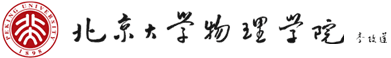
\includegraphics[width=.75\linewidth]{../PKUPhy}}
	}
	% Separator
	\newcommand{\newparagraph}{\pagebreak[3]\noindent%
		\hfil
		~\raisebox{-4pt}[10pt][10pt]{\decofourright~~~~~~~~\decofourleft}~ %
		\par
	}
%	% Background % Use when necessary
%	\usepackage{background} %Waterstamp package
%	\SetBgContents{...的实验报告} %Waterstamp to prevent copying
%	\SetBgScale{5} %Waterstamp setting
	% Essay format
	\renewcommand\appendixname{附录}
	\renewcommand\abstractname{}%摘要
	\renewcommand\tablename{表}
	\renewcommand\figurename{图}
	\renewcommand\refname{参考文献}
	\makeatletter
	\def\@pacs@name{\songti\zihao{-4}{\bf PACS码:}}
	\def\@keys@name{\songti\zihao{-4}{\bf 关键词:}}
	\def\Dated@name{日期:}
	\def\Received@name{\zihao{-5}{接收} }
	\def\Revised@name{\zihao{-5}{修订} }
	\def\Accepted@name{\zihao{-5}{采纳} }
	\def\Published@name{\zihao{-5}{发表} }
	\makeatother
	\linespread{1.5}
	\renewcommand{\labelenumi}{\alph{enumi}.}
	\leftmargini=20mm
	\newcommand{\supercite}[1]{\textsuperscript{\,%
		[\citenum{#1}]}}
	\let\fancycite\cite
	\renewcommand{\cite}[1]{\textup{\fancycite{#1}}}
	% Math line spacing
	\newlength{\djot}
	\setlength{\djot}{\jot}
	\newcommand{\restorejot}{\setlength{\jot}{\djot}}

%Miscellaneous
%	\newcommand{\tabindent}{\hspace{2em}}
%FourierTransform
	\newcommand{\fourierf}{\mathscr F}
\begin{document}
%Basic Data
	\title{%
	\texstringonly{\hfil\\[2\baselineskip]}
	\sf\LARGE%
		He--Ne气体激光及其放电条件的研究%
	\texstringonly{\vspace{3ex}}}
	\author{\fangsong\large%
		Bryan%
	\vspace{2mm}}
	\affiliation{\it%
		北京大学物理学院~~学号:\normalfont 1500000000\,}
	\date{\today}
	\keywords{受激辐射,激光,He--Ne激光器,气体放电}
	\email{guesswhat@email.addr;}

\begin{abstract}
\vspace{10mm}
\begin{spacing}{1.5}\normalsize
\setlength{\parskip}{.3\baselineskip}
%	200—300字,
%	说明用什么方法做了什么事,
%	由此得到什么结果和结论,
%	有何意义.
%	不用缩略词,不用第一人称.
%%%%%%%%%%%%%%%%%%%%%%%%%%%%%%%%
%
%	实验中观察的样品为结构已知的高定向热解石墨(Highly oriented pyrolytic graphite, HOGP);本实验通过比较STM所成图像与样品实际结构,粗略地校准了STM的探针控制系统,从而使其能较为精确地获得结构未知样品的原子分辨像。
	激光作为受激辐射效应的直接应用,在理论和实验的研究中均有重要的意义。其中,具有代表性的He--Ne激光器作为一种制造相对简单、单色性好、工作稳定的气体激光器,在各领域均有广泛的应用,其基本原理和放电条件值得探究。
	
	本实验通过配置He--Ne混合气体,实现气体放电并产生激光,以此验证激光的基本原理。在此基础上,测量He--Ne激光器在不同的工作气压下放电电流与输出光功率的关系,探索了其较优的放电条件及背后的相关机理。
\end{spacing}
\end{abstract}

\maketitle
\thispagestyle{titlepagestyle}
%
%	\item 课程实验报告应假定读者既不是已知全部实验细节的指导教师,也不是缺少专业知识的公众,而是同领域的实验研究者,或审稿人. 不能要求读者要在读过课程讲义后才能读懂课程实验报告.
%	\item 公式、图和表要分别用阿拉伯数字编列序号. 公式和图表要达到可发表的质量.
%	\item 凡不是自己独立思考得到的内容都应该引参考文献. 不能大段引用同一参考文献. 对复杂问题,应该优先考虑引用参考文献得到结果. 对简单一些的问题才鼓励独立思考.
%	\item 较长的推导和说明可以作为附件提交,不占用报告篇幅.
%	\item 思考题不是报告的组成部分. 应另起一页附在报告的最后.
\section{引言}
%%	研究论文引言一般包含以下内容:
%%	(1)所研究领域背景和现状;
%%	(2)有待研究的问题;
%%	(3)本研究的目的、主要内容和结果;
%%	(4)结果的意义.\par
%%	在写实验报告的引言时,同学可以假想自己是第一个做类似研究的人.\par
%%	引言一定要切合报告正文,不能漫无目的地介绍背景. 要快速地将读者引导到报告主题上,并作较深入的讨论.\par
%%	引言篇幅可以在较大范围内变化,但最长不应超过报告文字篇幅的1/3.\par
%%	引言撰写可以参考实验讲义,可以复述,但不能复制讲义上的任何一句话.\par
%%%%%%%%%%%%%%%%%%%%%%%%%%%%%%%
	1917年前后,爱因斯坦(A. Einstein)首先在旧量子论的框架内描述了原子的受激辐射\supercite{einstein1917quantentheorie}。人们猜想这一现象可用于加强光场,这便是激光,即\textit{受激辐射光放大}(Light Amplification by
	Stimulated Emission of Radiation, LASER or laser)之起源。
	
	1957年,贝尔实验室(Bell Labs)的查尔斯·汤斯(C. H. Townes)和阿瑟·肖洛(A. Schawlow)在利用氖光灯照射稀土晶体时,首先观察到了晶体产生的激光\supercite{schawlow1958infrared}。事实上,在此之前,\textit{微波放大}(Microwave Amplification by Stimulated Emission of Radiation, MASER or~maser)已经实现,并对激光的设计带来了很大的启发\supercite{townes1999laser}。
	
	在波长 \SI{632.8}{\nm} 可见光区工作的He--Ne气体激光器同样由贝尔实验室于1962年开发,这是目前应用最为广泛的激光器之一\supercite{white1962continuous}。本次实验尝试通过合理配比He--Ne气体,以气体放电激励实现激光输出,即重现 \cite{white1962continuous} 的实验结果;在此基础上,探究气体压强等因素对输出光功率的影响,检验相应的经验规律,对气体激光的原理及进一步优化设计提供一定的参考。
\section{理论}
	当原子处于激发态$E_2$时,如果恰好有能量为$(E_2-E_1)$的光子入射,在入射光子的影响下,原子会发出一个同样的光子而跃迁到低能级$E_1$上去,这便是受激辐射(stimulated emission)。这里,\textit{“同样”}意味着受激辐射发出的光子和外来光子的频率、相位、传播方向以及偏振状态全同。
	
	如今,利用薛定谔方程及含时微扰的办法,可以更为严谨地导出受激辐射现象;参见 \cite{griffiths2016introduction}, \CJKunderdot{单个}原子在外场下受激辐射与吸收光子的概率实际上是等同的。然而,对于处在平衡态的大量原子而言,相应能态上的粒子数遵循统计分布;事实上,粒子数目随能态增高而指数地减少,即:\vspace{-2ex}
	\begin{equation}
		E_2 > E_1,\quad N_2 \ll N_1
	\end{equation}
	
	因此,对一个由大量原子组成的纯粹的二能级系统而言,虽然存在受激辐射,但其发生的概率远小于吸收,不能产生激光。由此可见,产生激光的前提和关键在于\textbf{粒子数反转},即设法使$N_2 > N_1$并维持如此。更细致的分析还应考虑统计分布导致的权重;一般来说,要求:
	\begin{equation}
		\frac{N_2}{g_2} > \frac{N_1}{g_1}
	\end{equation}
	$g_{1,2}$即为统计权重。
	
	本实验考察的He--Ne混合气体中,实际产生激光(发生受激辐射)的是Ne原子,He原子则起\textit{传递能量}的作用,以实现粒子数反转;具体流程如图 \ref{fig:HeNeLevel} 所示。
	\begin{figure}[!h]
	\centering
	\vspace{-1.2\baselineskip}
	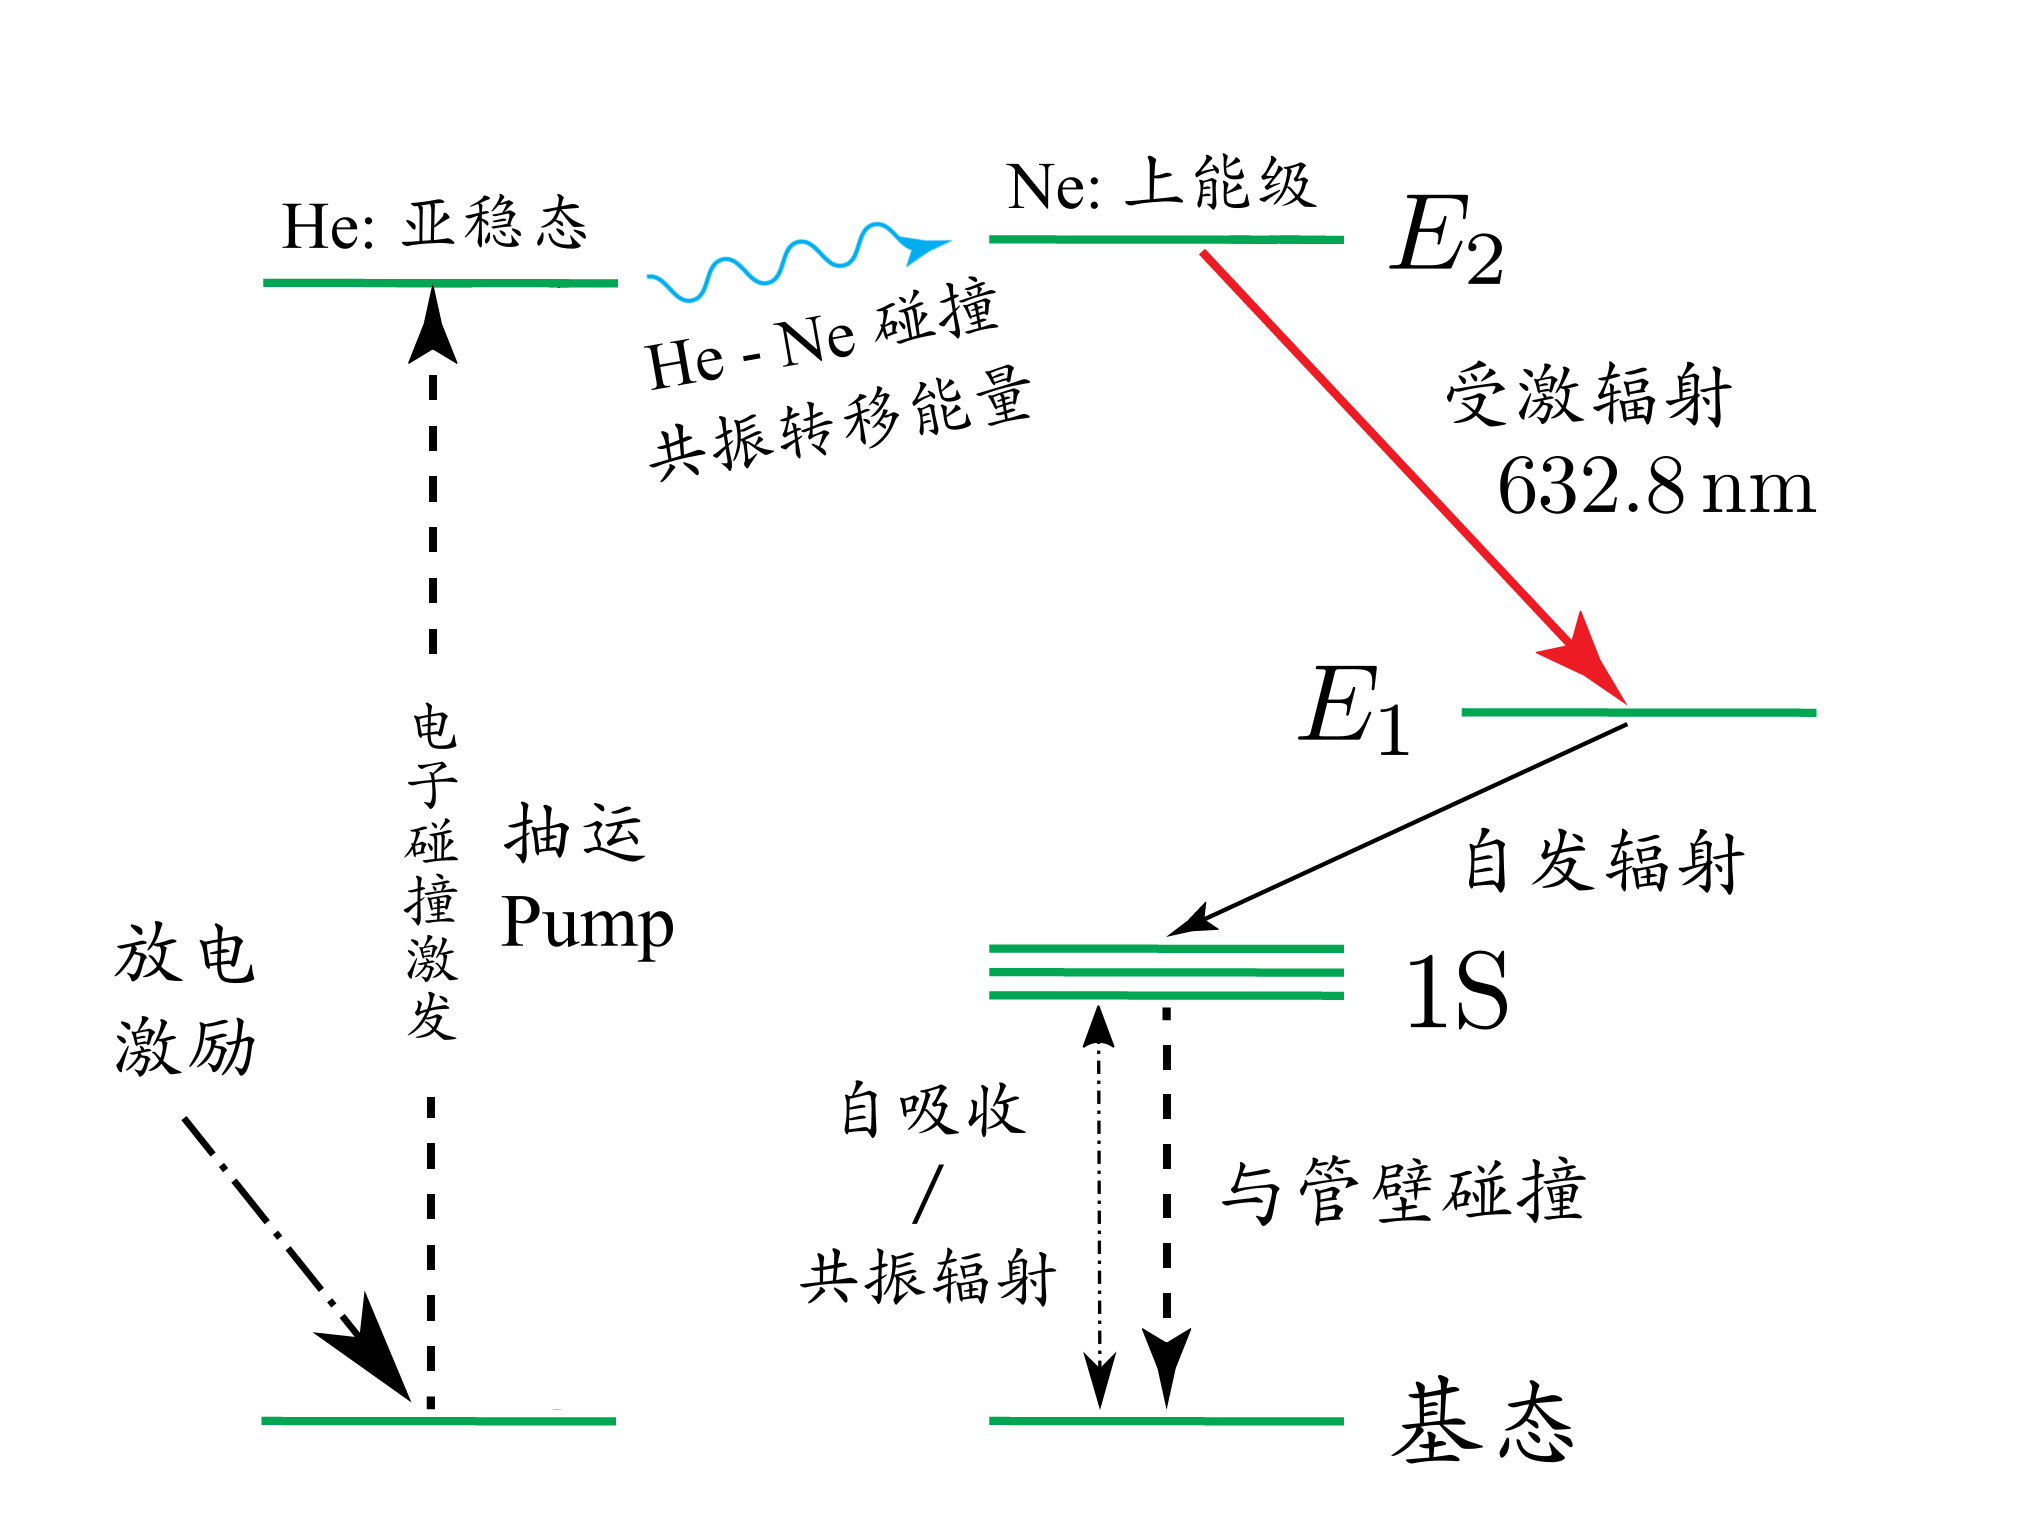
\includegraphics[width=.8\linewidth]{HeNeLaserLevel.png}
	\caption[\textup{He--Ne}激光原理]{%
		\textup{He--Ne}激光发生过程的能级示意图\footnote{%
			图像据网络资源修改得到:\par
			\noindent%\fontsize{9pt}{\parskip}%
			\url{https://en.wikipedia.org/wiki/File:HeNe_Laser_Levels.png}%
		},参考 \cite{textbook}. \\[1ex]
		注:示意图中的能级间隔不全按照比例,但相对高低与实际一致;\\
		\textup{He}的亚稳态($2^1\mrm{S}_0$)与\textup{Ne}的上能级($3\mrm{S}_2$)实际十分接近,图中夸大了两者的差距。\\
		另外,图中仅体现了 \SI{632.8}{\nm} 的受激辐射。
		\vspace{1ex}
	}
	\label{fig:HeNeLevel}
	\end{figure}
\FloatBarrier
	
	这里应当注意,图 \ref{fig:HeNeLevel} 中的中间能态$1\mrm{S}$中存在亚稳态,同时$1\mrm{S}$跃迁至基态发出的共振辐射容易被别的基态Ne原子吸收,即发生\textit{自吸收}过程\supercite{textbook};这相当于延长了$1\mrm{S}$态的寿命,导致处在该低能态的粒子数目较多,不利于维持粒子数反转。相应的解决办法是:设法增大气体容器的管壁面积,使处在$1\mrm{S}$态的Ne原子与管壁碰撞回到基态。因此,本实验中的气体放电在\textbf{毛细管}中进行。
	
	此外,He--Ne混合气体的受激辐射频率并非只有 \SI{632.8}{\nm}; 事实上,最早实现的He--Ne气体激光器正是工作在红外波段(\SI{1.15}{\um},参见 \cite{javan1961population})。同时,单个谱线还存在一定的展宽,这也应当加以考虑。综上所述,有必要使用光学\textbf{谐振腔}进行选频、增强;本实验中使用的光学谐振腔结构如图 \ref{fig:gasTube} 所示。
	\begin{figure}[!h]
	\centering
	\vspace{-.5\baselineskip}
	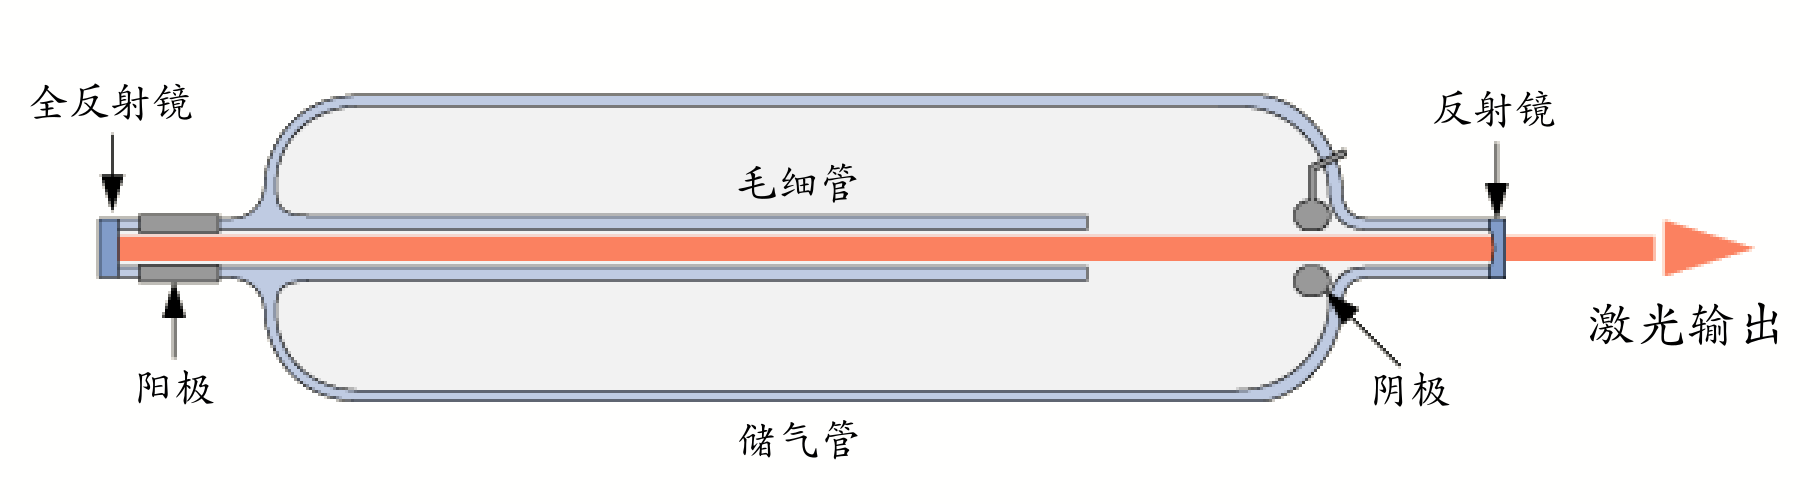
\includegraphics[width=.9\linewidth]{gasTube.png}
	\caption[\textup{He--Ne}激光管结构]{%
		\textup{He--Ne}激光管结构示意图\footnote{%
			图像据网络资源修改得到:\par
			\noindent%\fontsize{9pt}{\parskip}%
			\url{https://en.wikipedia.org/wiki/File:Hene-1.png}%
		},本实验中毛细管直径$d\sim\SI{1.25}{\mm}$. \vspace{1ex}
	}
	\label{fig:gasTube}
	\end{figure}
\FloatBarrier
	
	对于放电条件,这里引用 \cite{textbook} 给出的若干\textbf{经验规律}:
	\begin{enumerate}[noitemsep]
	\item 最佳He--Ne配比约为$7:1$; 
	\item 气体总压强$p\sim\SI{300}{\Pa}$时,输出光功率接近最大;
	\item 固定总压和气体配比,存在一个最佳放电电流,此时输出光功率最大。
	\end{enumerate}
	本实验中,调整相应参数在以上建议值附近,进而对其有效性进行粗略的检验。
\section{实验装置}
%%	在此部分需要将实验条件交待清楚到别人能重复你的实验结果的程度. 此外,还需表明你已尽了最大努力来提高实验精度和结果的可靠性. 简单的不确定度估计可以在此节给出,复杂一些的可以放到分析讨论部分.\par
%%	实验条件不仅是指直接影响实验结果的实验参量,而且还包括影响实验质量和可靠性的因素,如室温、空气湿度、基真空、原材料纯度等.\par
%%	作为教学实验报告,此节写详细一点没有坏处.\par
%%	成段有叙述,必要才分节。
%%%%%%%%%%%%%%%%%%%%%%%%%%%%%%%
	本实验依赖纯净的气体环境,以实现He, Ne原子之间高效的能量传递,杜绝不必要的碰撞损耗或碰撞激发。因此,实验中采用标识纯度高达99.999\%的He气和Ne气,且应当去除系统中的空气,以排除干扰。
	
	\begin{figure}[!h]
	\centering
	\vspace{-.5\baselineskip}
	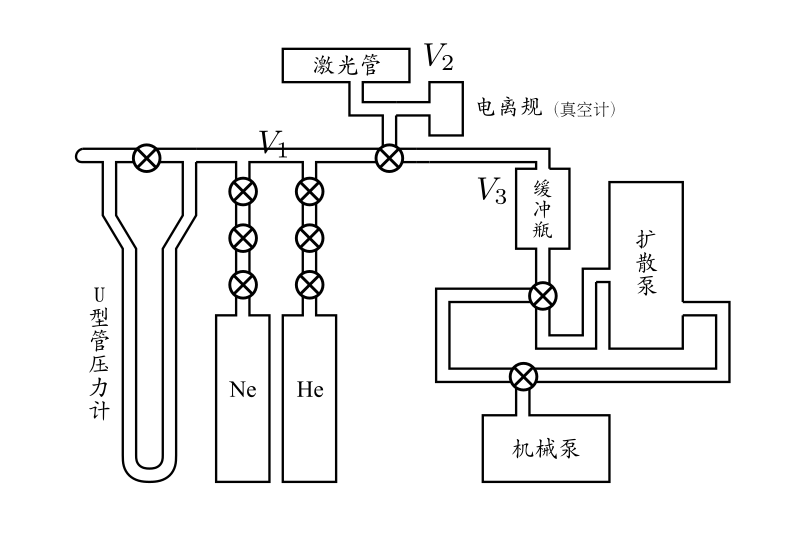
\includegraphics[width=.9\linewidth]{app.png}
	\vspace{-3ex}
	\caption[实验真空系统]{%
		实验使用的真空系统结构示意图\footnote{%
			图像据网络资源修改得到:\par\vspace{-.8ex}
			\noindent\fontsize{7pt}{\parskip}%
			\url{https://github.com/chaserhkj/ModPhyLab/raw/master/Research_on_the_discharge_conditions_of_He-Ne_gas_laser/graph2.pdf}%
		},参考 \cite{textbook}.\\[1ex]
		$V_{1,2,3}$为阀门之间的容积;
		实验中首先对$V_1$充\textup{He}气,
		再分别令其膨胀至$V_2,V_3$, \\[.3ex]
		考察压强的相对变动,得到比值
		$V_1 : V_2 : V_3 \sim 1 : 2.6 : 1.9$. \vspace{1ex}
	}
	\label{fig:app}
	\end{figure}
\FloatBarrier
	
	由此可见,本实验强烈依赖真空技术以实现气体配比和压强控制。
	\begin{enumerate}
	\item \textbf{抽空}:首先使用\textbf{机械泵},逐步打开联通系统各部分的阀门,逐段排空系统中的气体;机械泵工作若干分钟后,气压降至 \si{\Pa} 量级,此时可启用\textbf{电离真空计}\footnote{仪器型号:DL-5型程控真空计}以监测真空度。确认有$p\sim\SI{1}{\Pa}$后,启用\textbf{扩散泵},进一步抽气至$\SI{e-3}{\Pa}$量级。本实验中,最终抽空至压强$p = \SI{4.0e-3}{\Pa}$. 
	\item \textbf{配气}:充入的气体压强在 \SI{100}{\Pa} 量级,超过电离真空计的量程;故此后关闭电离规,使用U型管气压计确定气体压强,如图 \ref{fig:app} 所示。考虑理想气体状态方程:$pV = nRT$, 充分利用与气瓶相连的多级阀门,结合相互独立又可两两联通的空间$V_1,V_2,V_3$, 对充入气体的量进行调配。结果如表 \ref{tab:mixGas} 所示。
	\end{enumerate}
	
	\begin{table}[!h]
	\centering
	\caption[配气表格]{\textup{He--Ne}气体配比过程及相应参数;\\
		其中$h$是\textup{U}型管气压计的液面高差,压强$p = \rho gh,\,
			\rho = \SI{1.09}{g/\cm^3}$. }
	\begin{tabularx}{.85\linewidth}{C{.45}C{1}C{.8}C{.9}C{.9}}
	\toprule\midrule
		\multirow{2}{*}{步骤} &
		\multirow{2}{*}{气体} &
		\multirow{2}{*}{占据体积} &
		\multicolumn{2}{c}{压强} \\
	\cmidrule{4-5}
		& & & $h / \si{\cm}$ & $p / \si{\Pa}$ \\
	\midrule
		(1) & He & $V_2$ & 7.3 & 780 \\
		(2) & Ne & $V_1$ & 2.8 & 299 \\
		(3) & He--Ne 混合 & $V_1 + V_2$ & 6.0 & 641 \\
	\midrule\bottomrule
	\end{tabularx}
	\label{tab:mixGas}
	\end{table}
\FloatBarrier
	
	利用表 \ref{tab:mixGas} 的结果,我们可以计算He--Ne配比;事实上,有:
	\begin{equation}
	\begin{gathered}
		p_{(1)} V_2 = n_{\textup{He}} RT,\\
		p_{(2)} V_1 = n_{\textup{Ne}} RT,\\
		p_{(3)} (V_1 + V_2)
			= (n_{\textup{He}} + n_{\textup{Ne}}) RT,
	\end{gathered}
	\end{equation}
	这里我们视$V_1/V_2$为未知量,以保证结果的较高精度;解得:
	\begin{equation}
		\frac{V_2}{V_1} \approx 2.46,\quad
		\frac{n_{\textup{He}}}{n_{\textup{Ne}}}
			\approx 6.42
	\end{equation}
	
	至此,我们便完成的气体的配比,得到了He--Ne比约为6.42的混合气。在此基础上,利用带安培计的专用电源\footnote{仪器型号:JD-2型He--Ne激光电源}给电极加压直至气体放电,利用光功率计\footnote{仪器型号:FD-LPM-A型激光功率计}检测输出激光强度,开始测定。
\section{结果与分析}
%	实验结果应尽量以图表的形式给出. 每一个图表都应该是完整的,即阅读图表时可以不必依赖正文.\par
%	依自己意愿,实验结果和对结果的分析讨论既可分为两节也可合在一节.\par
%
%	每个图一般包含:图名、轴名、轴、刻度、标尺、数据点、曲线、图例、标注和图注等部分. 应尽量让读者不看正文就能基本理解图的含意.\par
%	逐点测量得到的函数关系要同时用表格和图给出. 需要作比较的多条曲线要画在同一图上.\par
%	为避免读者在图表和正文间反复跳跃阅读,在正文中也要对图表作必要的说明.\par
%
%	对于预料之外的实验结果,必须首先小心证明其可靠性.读者只有在相信你的实验结果时才愿意花时间看你的分析.\par
%	必须用文字归纳整理出正式的实验结果或结论.可信的实验结果是课程报告最重要的内容.作为一个实验物理工作者,分析解释出错并不丢脸,实验结果不被采信则是致命的.\par
%	教学实验的结论往往是预先知道的. 所以,教师更关心的是你的说理过程. 一般说来,单由课内实验的结果不足以能得到明确的结论. 此时,你可以引用他人的研究结果来帮助帮助自己的论证,但必须注明出处. \par
%	确实不能得到明确结论时,可以给出几种可能结论并指出可以再做哪些实验来帮助作进一步的判断.\par
%	总之,分析讨论部分要做到: 论据要valid,论证要reasonable,结论要convincing.\par
%%%%%%%%%%%%%%%%%%%%%%%%%%%%%%
	缓慢增加激光管两端的电压,直到激光管突然被点亮,发出漂亮的红光;实验现象如图 \ref{fig:photo} 所示,此时电流表、光功率计均出现非零示数。标志性的 \SI{632.8}{\nm} 红色光束表明,气体激光放电初步成功。
	\begin{figure}[!h]
	\centering
	\vspace{.2\baselineskip}
	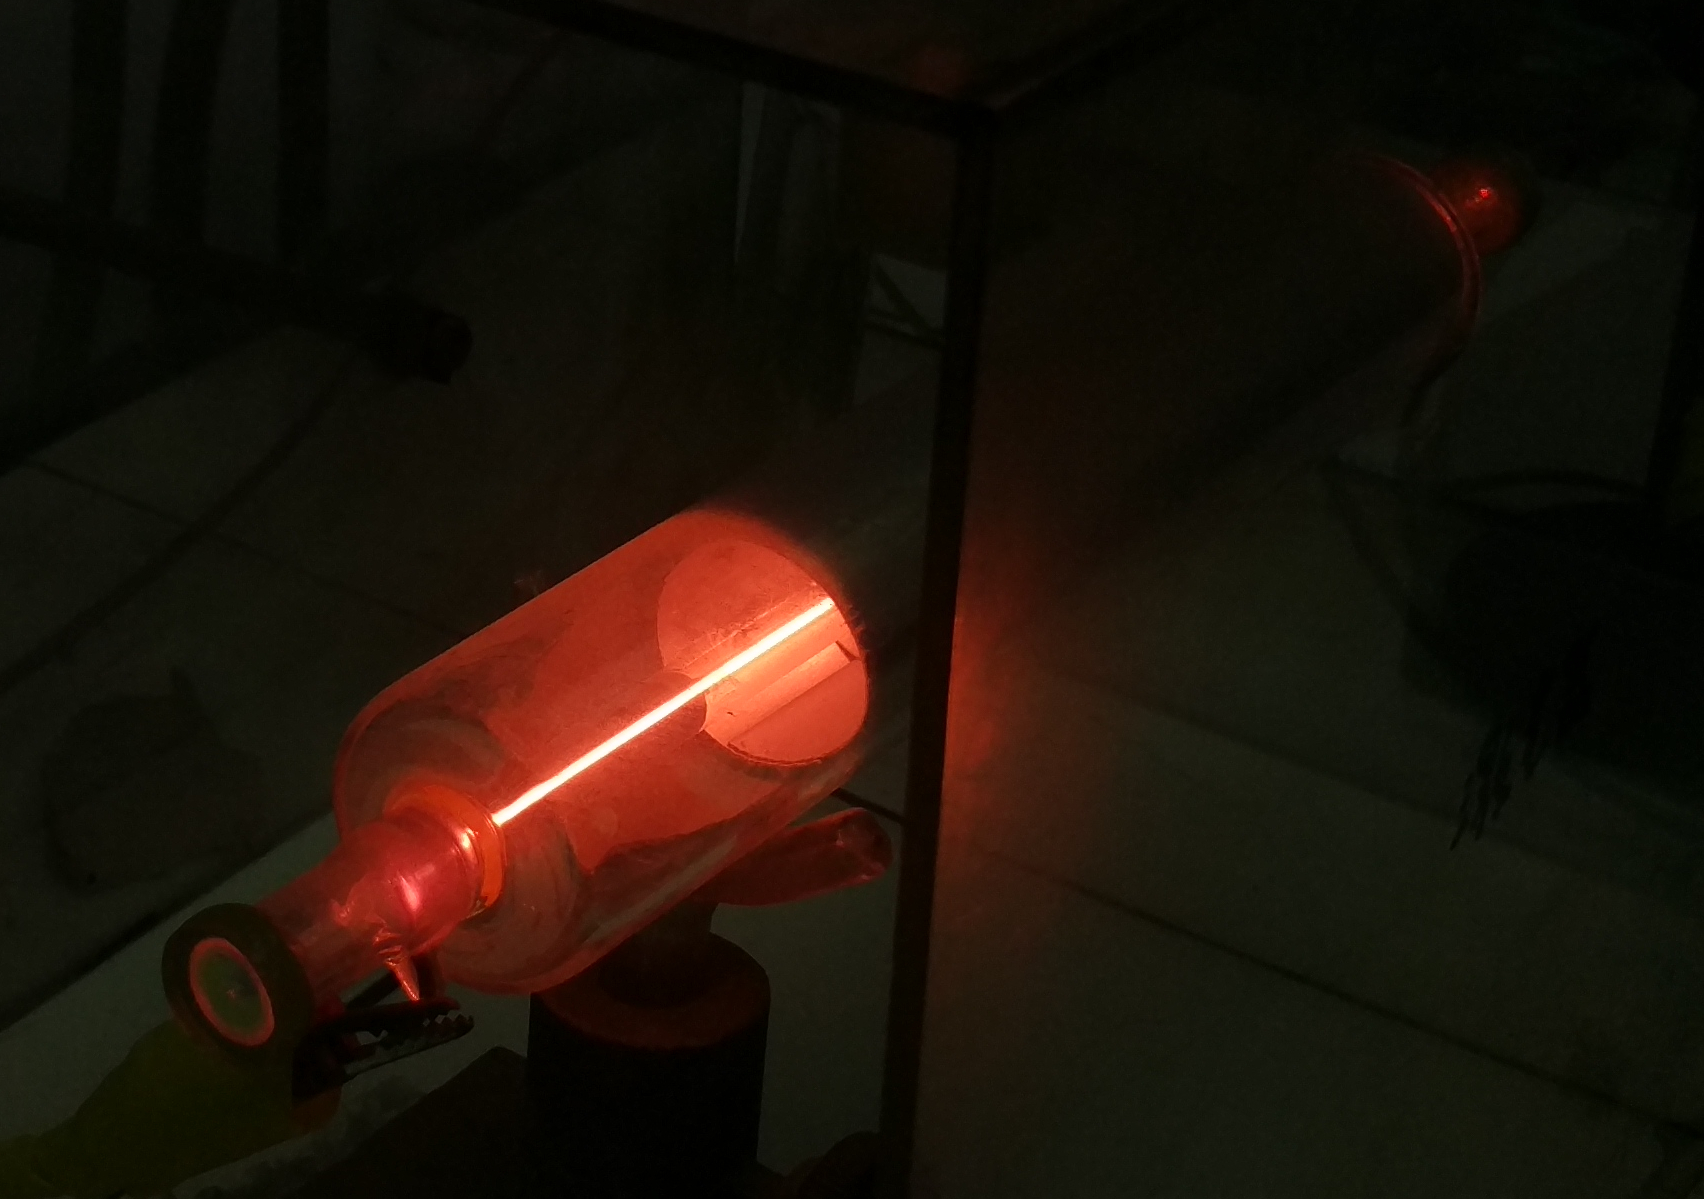
\includegraphics[width=.75\linewidth]{laser.jpg}
	\caption[激光管放电现象]{激光管放电现象——实验照片}
	\label{fig:photo}
	\end{figure}
\FloatBarrier
	
	调整所加电压,记录光功率随电流的变化关系;观察到,随着放电电流增大,输出光功率先增后减。放去部分气体,即降低总压,但保持He--Ne比例不变,重复上述实验并记录,结果综合于图 \ref{fig:powerVamp}. 
	
	记录数据的过程中,我们注意到,激光输出功率有不小的起伏。这一起伏的大小在图 \ref{fig:powerVamp} 中的误差棒上得以体现。该现象令我们联想到经典的\textbf{弗兰克--赫兹实验}(Franck–Hertz experiment),这一实验同样涉及气体放电,且在测定放电电流随电压变化的过程中,同样出现了类似的不稳定情况。
	
	\begin{figure}[!h]
	\centering
	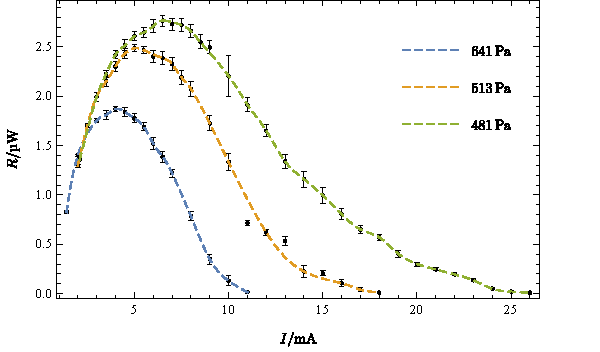
\includegraphics[height=.36\linewidth]{plotPowerAmp1.pdf}\\[1.5ex]
	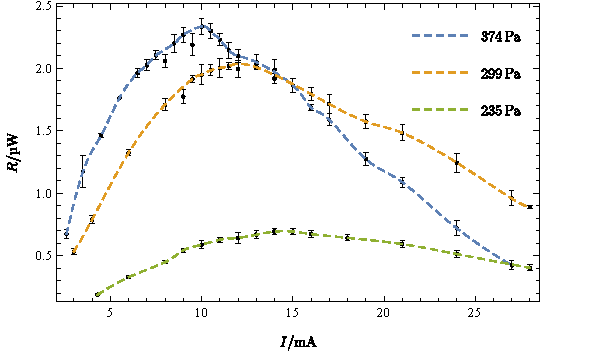
\includegraphics[height=.36\linewidth]{plotPowerAmp2.pdf}\\[1.5ex]
	\hspace{0em}
	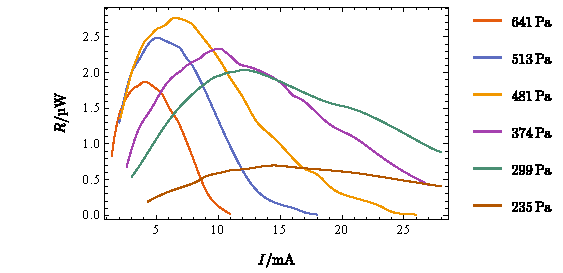
\includegraphics[height=.42\linewidth]{plotPowerAmpAll.pdf}
	\caption[输出功率变化曲线]{在不同气压$p$下测得的\textup{He--Ne}激光器输出功率与放电电流之关系曲线;\\[.8ex]
		其中,总气压$p$已在图例中标明;为使图像简明清晰,\\
		将6个$p$值对应的散点拆分绘制在第一、第二这两张图中,
		曲线汇总于第三图;\\
		趋势线为三阶插值曲线,在除去少量严重偏离的数据点后绘制得到。}
	\label{fig:powerVamp}
	\end{figure}
\FloatBarrier
	
	在此基础上,我们推测本实验中光功率起伏的可能根源为:
	\begin{enumerate}
	\item 气体放电是一个非平衡态;从改变所加电压到系统抵达稳恒状态,这一过程需要一定的\textbf{响应时间};本实验中读取数据时,系统可能尚未稳定,自然导致输出的光功率存在起伏;
	\item 宏观的光功率大小是受激辐射、吸收等一系列过程之贡献的统计平均结果;对于这一系统,可能存在显著的\textbf{涨落},需要利用统计物理的手段进一步分析;
	\item 可能还有\textbf{未考虑的变量}对系统的表现造成了不可忽略的影响;例如,本实验中并没有控制系统的温度恒定;而激光器长期点亮后,气体温度显著升高,这对结果势必会造成影响。
	\end{enumerate}
	实际原因可能是上述的综合,需要进一步研究加以确定。
	
	\newparagraph
	下面我们结合 \ref{fig:powerVamp} 检验 \cite{textbook} 给出的经验规律:
	\begin{enumerate}
	\item 本实验在He--Ne比约为6.42时获得了不错的激光输出,这一比值与建议值$7:1$比较接近,这便\textit{初步}验证了建议值的有效性;
	\item 随着总压强$p$不断减小,输出的光功率先增后减;本实验中,最大光功率对应的压强为 \SI{481}{\Pa}, 高于建议的 \SI{300}{\Pa}. 实际上,如图 \ref{fig:powerVamp} 所示,最佳$p$值可能在 \SIrange{374}{513}{\Pa} 之间,这一范围比建议值略偏大,但可以算是大致吻合。由于本实验的He--Ne比并不恰为$7:1$, 这也可能对最佳$p$值的大小造成影响;
	\item 固定总压和气体配比,输出光功率随电流先增后减,这一规律在图 \ref{fig:powerVamp} 中显而易见,得到验证。
	\end{enumerate}
	
	由此我们得到,\cite{textbook} 给出的经验规律基本可靠,这对进一步的实验改进指明了方向。同时我们还发现了如下规律:\textbf{激光输出功率峰值对应的放电电流随总压的减小而增大}。分析其物理根源,我们推测,这是因为最佳电流对应着Ne原子处于上能级的粒子数接近\textbf{饱和},而气体总压强越小,代表着气体越稀薄,就越需要更高的电子流密度才能达到饱和。
\section{结论}
%%	首先要给出实验结果,然后再给出由实验结果分析得到的结果和结论.此部分给出的内容要比摘要中的全面,用词要更准确.\par
%%%%%%%%%%%%%%%%%%%%%%%%%%%%%%
	本实验中,我们通过配置He--Ne比约为6.42的混合气体,实现了气体放电、激光输出;在此基础上,我们检验了He--Ne气体的其他放电条件,确认了输出光功率分别随气体总压强和放电电流先增后减的变化规律,为进一步获得更为优化的He--Ne激光器件创造了条件。
\section{致谢}
%	此部分感谢同组人...和对实验和报告有帮助的人.
%%%%%%%%%%%%%%%%%%%%%%%%%%%%%%
	在此前的物理实验中,我们已经多次使用了激光光源,并对其良好的特性有所了解。能够在本次实验中亲手创造出经典的 \SI{632.8}{\nm} 激光,这不能不说是十分震撼的。
	
	感谢与我合作的黄金锁同学,尤其感谢他在配气和记录时的出色工作;感谢耐心的荀坤老师给我们带来的巨大帮助。

\setlength{\bibsep}{2pt}
\linespread{1.2}\selectfont
\bibliographystyle{../BibStyle/gbt-7714-2015-numerical}
\bibliography{../BibStyle/Textbook,bib/Ref}

\clearpage
\end{document}
